\documentclass[journal,12pt,twocolumn]{IEEEtran}
\usepackage[utf8]{inputenc}
\usepackage{graphicx}
\usepackage{amssymb}
\usepackage{amsmath}
\title{Assignment 1}
\author{Kotikalapudi Karthik \\
CS21BTECH11030}

\begin{document}

\maketitle

\section*{ICSE 2018 Question 9 (c)}
\begin{figure}[ht!]
	  \centering 
	  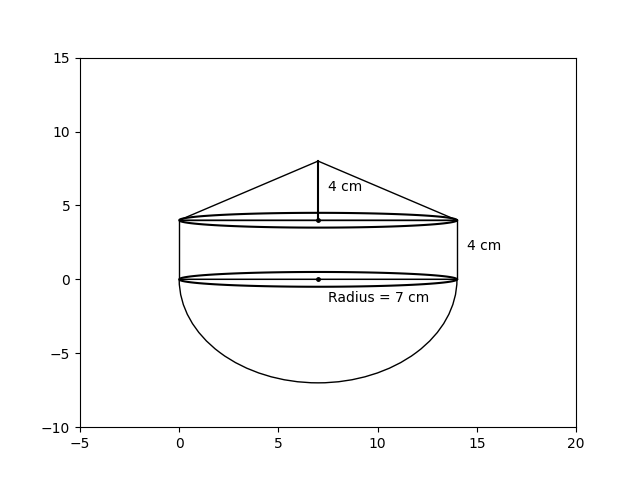
\includegraphics[width=\columnwidth]{Figs/question9c.png}
\end{figure}
\textbf{Solution :}\\
The various parameters considered in this problem are listed in Table
\eqref{table:Table1}
\begin{table}[ht!]
    \centering
    
\begin{tabular}{|c|c|c|}
\hline
 Symbol & Value & Description \\
\hline
 $r$  & $7cm$  & radius of cone, cylinder and hemisphere  \\
 \hline
 $h$  & $4cm$  & height of cone and cylinder  \\
\hline
$V1$ & $\frac{1}{3} \pi r^2 h$ & Volume of cone\\
\hline
$V2$ & $\pi r^2 h$ & Volume of cylinder\\
\hline
$V3$ & $\frac{1}{3} \pi r^3$ & Volume of hemisphere\\
\hline
$V$ & ? & Volume of the figure\\
\hline
\end{tabular}
    \caption{}
    \label{table:Table1}
\end{table}

From the given information, the volume of the figure is equal to the sum of the volume of the cone, cylinder and hemisphere. Thus,\\
$V$ = $V1 + V2 + V3$\\
$\implies V = \frac{1}{3} \pi r^2 h + \pi r^2 h + \frac{2}{3} \pi r^3$

\begin{align*}
    \therefore V&= \frac{2}{3} \pi r^2 (2h+r)\\
    \text{By substituting $h$ and $r$,}\\
    \text{Volume of the figure}\\
    &= \frac{2}{3} 49 (8+7) \pi\\
    &= 490 \pi\\ 
    &\approx 1539.38cm^3
\end{align*}
\end{document}
